\documentclass[12pt,a4paper]{article}
\usepackage[utf8]{inputenc}
\usepackage[ngerman]{babel}
\usepackage{graphicx}
\usepackage{booktabs} % Für Tabellen
\usepackage{caption}
\usepackage{amsmath}
\usepackage{enumitem} % Paket für bessere Nummerierung
\usepackage{csquotes} 


\usepackage{tikz}
\usetikzlibrary{positioning}
\tikzstyle{block} = [rectangle, draw, fill=blue!20, text width=6em, text centered, rounded corners, minimum height=4em]
\tikzstyle{arrow} = [thick,-,>=stealth]



\usepackage[hypertexnames=false]{hyperref} % Hinzugefügte Option

\begin{document}
	
		
		% Titelseite
		\begin{titlepage}
			\begin{center}
				\vspace*{1cm}
				\Huge
				Sprache, Spracheingabe, Text \& Übersetzung mit Google Cloud APIs
				
				
				\vspace{1.5cm}
				\LARGE
				M.Sc. Onur Yilmaz
				
				\vspace{1.5cm}
				\Large
				Angewandte Künstliche Intelligenz
				
				\vfill
				
				Schriftliche Ausarbeitung - Cloud Computing
				\vspace{0.5cm}
				\large
				Fachhochschule Südwestfalen
				\vspace{0.8cm}
				\Large
				\\
				Gutachter: Prof. Dr. Giefers
				\\
				\vspace{0.5cm}
				\large		
				\today
			\end{center}
		\end{titlepage}

\thispagestyle{empty}
\tableofcontents

\newpage
\section*{Einleitung}
Im Rahmen dieser Arbeit werden verschiedene Technologien und Anwendungen im Bereich Sprache und Textverarbeitung vorgestellt, die auf den Diensten von Google Cloud basieren, einschließlich der \textit{Cloud Speech API}, der \textit{Cloud Translation API}, der \textit{Natural Language API} und der \textit{Text-to-Speech API} \cite{google}.
\\ \\
Im Abschnitt über die \textit{Grundlagen} wird eine Einführung in die Konzepte der API und des Umgangs mit dem Google Cloud Dienstes eingeganen.
\\ \\
Der Abschnitt \textit{Spracherkennung und -transkription} fokussiert sich auf die \textit{Cloud Speech API}, die die Transkription von Audio in Text ermöglicht, und die Methoden zur Messung und Verbesserung der Sprachgenauigkeit.
\\ \\
In der \textit{Sprachübersetzung} wird die \textit{Cloud Translation API} behandelt, die den Prozess der Übersetzung von Texten in verschiedene Sprachen ermöglicht.
\\ \\
Der Bereich \textit{Textanalyse} befasst sich mit der \textit{Natural Language API}, die Techniken zur Klassifizierung von Text in Kategorien und zur Analyse von Entitäten und Sentiments bietet.
\\ \\
Im Abschnitt \textit{Sprachsynthese} wird die \textit{Text-to-Speech API} vorgestellt, die die Erzeugung synthetischer Sprache ermöglicht.
\\ \\
Die Arbeit dient nicht nur als theoretischer Überblick, sondern bietet auch praktische Einblicke und Anleitungen zur Verwendung dieser Tools. Dabei werden unterschiedliche Schwierigkeitsgrade und Themenbereiche abgedeckt, um einen umfassenden Einblick in die Möglichkeiten der Sprach- und Textverarbeitung mit Google Cloud zu bieten.

	
\newpage

\section{Grundlagen}
\subsection{Was ist eine API}
Eine API (\textit{Application Programming Interface}) ist eine Schnittstelle, die es verschiedenen Softwareanwendungen ermöglicht, miteinander zu kommunizieren. Es handelt sich im Wesentlichen um eine Reihe von Regeln und Protokollen, die von den Entwicklern befolgt werden müssen, um auf die Funktionen eines Softwareprodukts zuzugreifen. APIs können in verschiedenen Formen existieren, wie z.B. Web-APIs, die über HTTP-Kommunikation arbeiten, oder als Bibliotheken und Frameworks für spezifische Programmiersprachen.

\subsection{Erstellen eines API-Schlüssels}
Ein API-Schlüssel ist ein eindeutiger Identifikator, der verwendet wird, um eine Anwendung zu authentifizieren, die auf die Funktionen einer API zugreifen möchte. Dieser Schlüssel dient als eine Art "Passwort", das sicherstellt, dass nur autorisierte Anwendungen Zugang zur API haben. Die genauen Schritte zum Erstellen eines API-Schlüssels können je nach Anbieter der API variieren, aber in der Regel beinhalten sie das Anmelden bei einem Entwicklerportal, das Erzeugen eines neuen Schlüssels über eine Benutzeroberfläche und das Kopieren dieses Schlüssels in die Anwendung, die die API nutzen wird.

\subsection{Erstellen und Aufrufen der API-Anfrage}
Um eine API-Anfrage zu erstellen, muss ein Entwickler eine HTTP-Anfrage (normalerweise GET oder POST) an die URL der API senden, zusammen mit allen erforderlichen Parametern und dem API-Schlüssel. Die Anfrage kann auch einen Anforderungskörper enthalten, der zusätzliche Daten zur Verarbeitung an die API sendet. Nach dem Senden der Anfrage wird die API diese verarbeiten und eine Antwort zurückgeben, normalerweise in Form einer JSON- oder XML-Datei, die die angeforderten Daten oder das Ergebnis der Verarbeitung enthält.

\subsection{Interaktion mit der Google Cloud API}

Der Prozess der Interaktion mit der Google Cloud API kann in vier grundlegende Schritte unterteilt werden:

\begin{enumerate}
	\item Der Entwickler sendet eine API-Anfrage von seiner Anwendung aus. Diese Anfrage enthält die erforderlichen Parameter und den API-Schlüssel. 
	
	\item Die Anfrage wird an die Google Cloud API gesendet, die auf einem Server von Google gehostet wird. Dies geschieht im Hintergrund durch die Netzwerkinfrastruktur und erfordert in der Regel keinen spezifischen Code.
	
	\item Die Google Cloud API verarbeitet die Anfrage. Dies kann beinhalten, dass sie auf Daten in einer Datenbank zugreift, Berechnungen durchführt oder andere Funktionen ausführt. Auch dies geschieht auf dem Server und ist für den Entwickler in der Regel nicht sichtbar.
	
	\item Die Google Cloud API sendet eine Antwort zurück an die Anwendung des Entwicklers. Diese Antwort enthält die Daten oder das Ergebnis, das der Entwickler angefordert hat.
	
\end{enumerate}
\begin{figure}[h!]
	\centering
	\begin{tikzpicture}[node distance=2cm]
		
		\node (developer) [block] {Entwickler sendet API-Anfrage};
		\node (api) [block, right of=developer, node distance=3cm] {Google Cloud API};
		\node (response) [block, below of=api, node distance=2cm] {API sendet Antwort};
		
		\draw [arrow] (developer) -- (api);
		\draw [arrow] (api) -- (response);
		
	\end{tikzpicture}
	\caption{Interaktion mit der Google Cloud API}
\end{figure}


\subsection{Erstellen eines API-Keys in Google Cloud}

Um einen API-Key in der Google Cloud Platform (GCP) zu erstellen, folgen wir diesen Schritten:

\begin{enumerate}[label=\textbf{\arabic*.}]
	\item \textbf{Einloggen und Projekt auswählen:} \\
	Wir melden uns in unserem Google Cloud Console-Konto an und gelangen auf die Dashboard Seite (siehe Abbildung 2):

	\begin{figure}[h!]
		\centering
		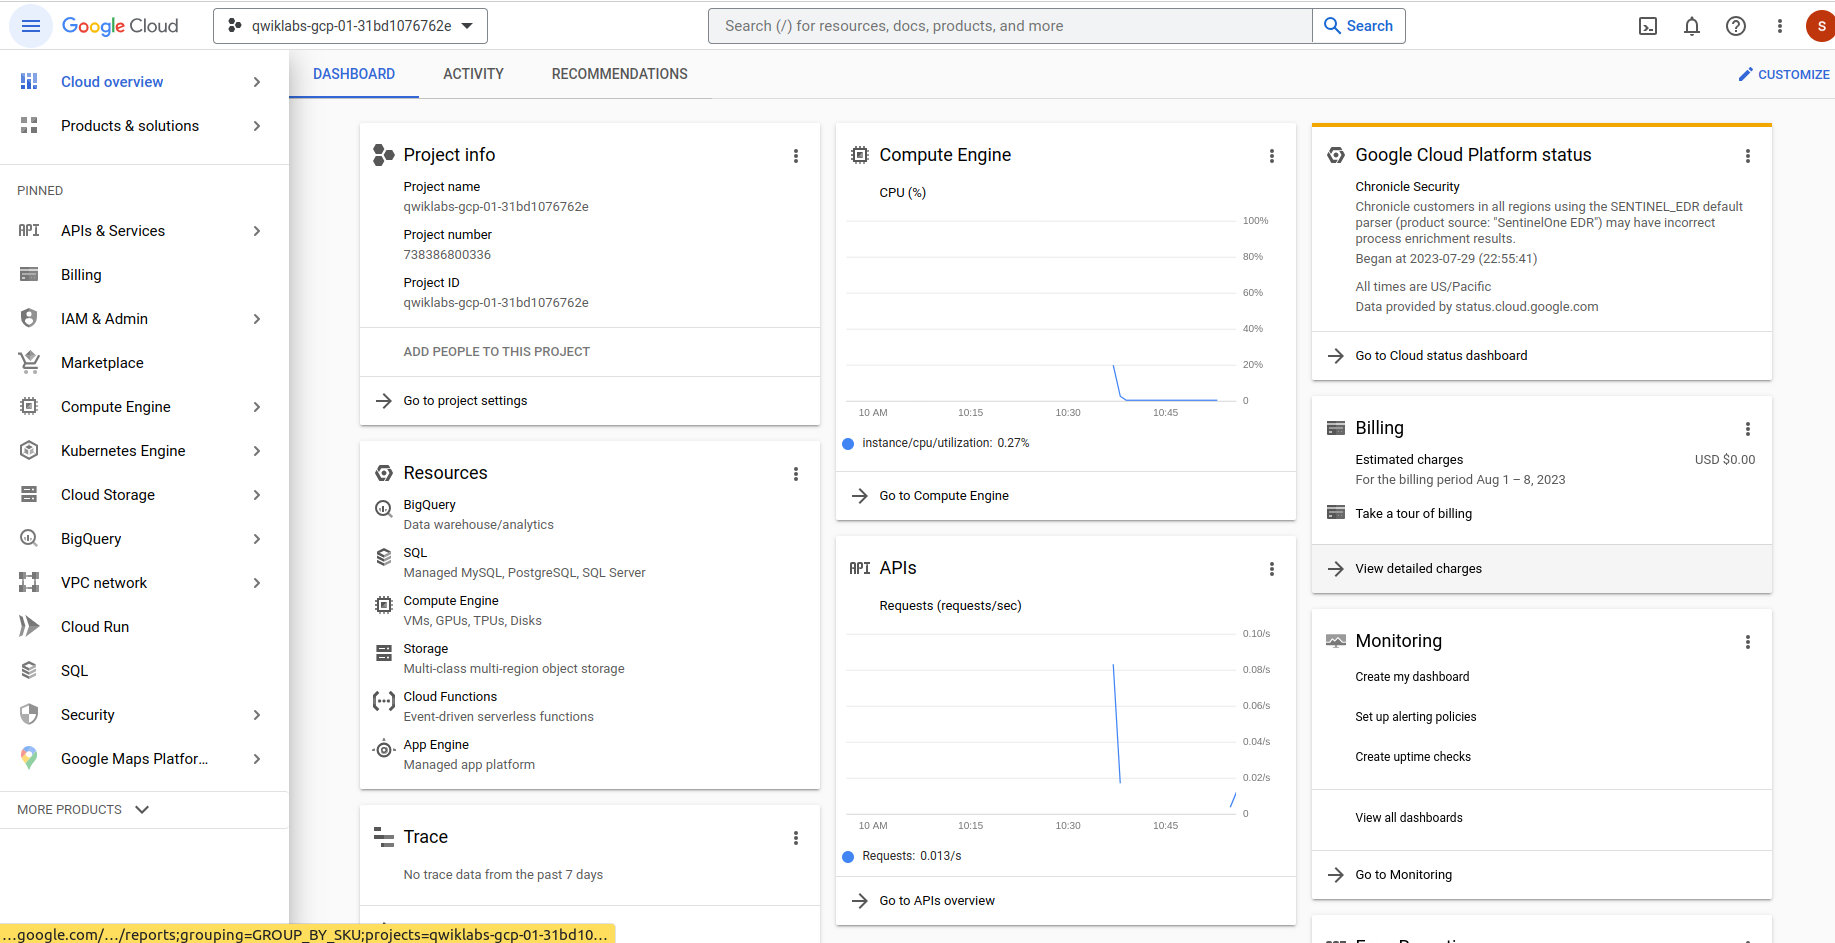
\includegraphics[width=1\linewidth]{../images/Dashboard}
		\caption{Dasboard GCP}
		\label{fig:dashboard}
	\end{figure}
\item \textbf{APIs \& Dienste Dashboard öffnen:} \\
Hier navigieren wir links auf den Reiter \enquote{APIs \& Dienste} und von dort aus auf \enquote{Credentials}. \\
 \item \textbf{Erstellung des API-Keys:} \\ 
 Nun klicken wir anschließend auf die Schaltfläche \enquote{+Create Credentials}, um den Prozess zur Erstellung eines neuen API-Keys zu starten.
\begin{figure}[h!]
	\centering
	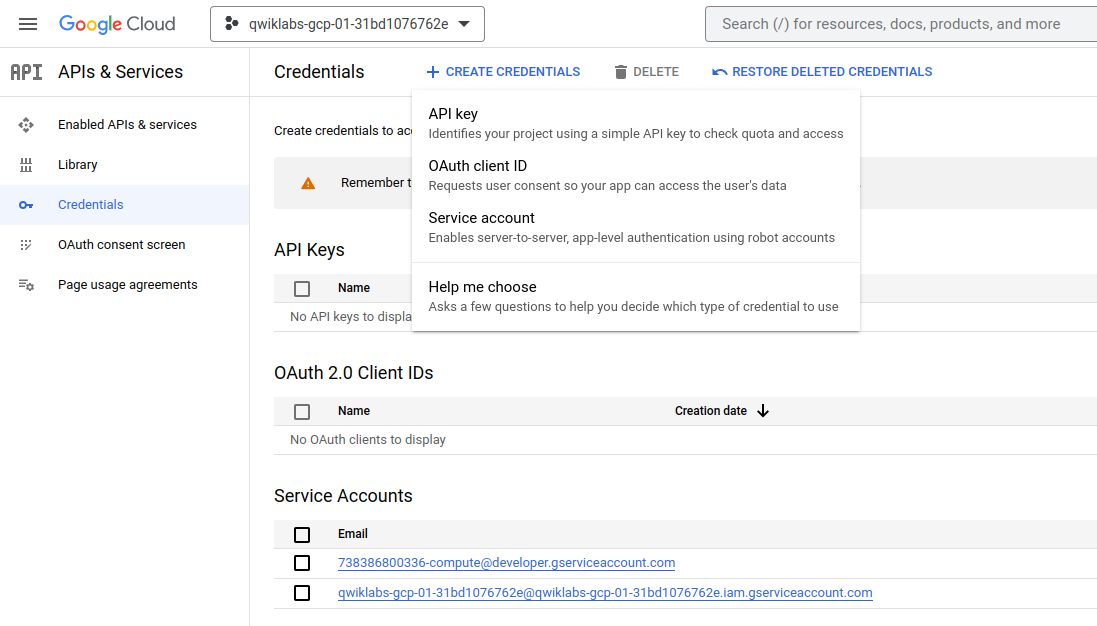
\includegraphics[width=0.8\linewidth]{../images/API}
	\caption{Erstellung eines API-Keys}
	\label{fig:api}
\end{figure}
\ \\
\item \textbf{API-Key - Konfiguration:} \\
Anschließend werden wir aufgefordert den zugehörigen API-Typ auszuwählen. Diesen passen wir nach unseren Anwendungen an. Wir können beispielsweise festlegen, welche APIs dieser Schlüssel verwenden darf.
\ \\
\item \textbf{Verwendung des API-Keys:} \\
Sobald der API-Key erfolgreich erstellt wurde, erhalten wir einen eindeutigen Schlüsselwert. 
\item \textbf{Verbindung zur Linux-Instanz per SSH:} \\
Wir verbinden uns über SSH mit der für uns bereitgestellten Linux-Instanz:
\begin{itemize}
	\item Klicken wir im Navigationsmenü (Symbol für das Navigationsmenü) auf \enquote{Compute Engine} $>$ \enquote{VM-Instanzen}.
\end{itemize}
\end{enumerate}

\newpage
\section{Spracherkennung und -transkription}
Die Spracherkennung und -transkription, auch als \textit{Automatic Speech Recognition} (ASR) bekannt, ist ein wichtiger Bereich der künstlichen Intelligenz und der Signalverarbeitung. In diesem Abschnitt werden wir uns damit beschäftigen, wie gesprochene Sprache in geschriebenen Text umgewandelt werden kann. Dieser Prozess wird als Transkription bezeichnet.
\subsection{Transkription von Sprache zu Text}
Die Transkription von Sprache zu Text ist das Verfahren, bei dem Audiosignale, die menschliche Sprache enthalten, analysiert werden, um den entsprechenden Textinhalt zu erzeugen. Dies kann in vielen Anwendungen nützlich sein, von automatischen Untertiteln für Videos bis hin zur sprachbasierten Interaktion mit virtuellen Assistenten.

\subsection{Schritte im Speech-to-Text Prozess}

Der Prozess der Sprache-zu-Text-Transkription kann in mehrere Teilschritte zerlegt werden, darunter:

\begin{enumerate}
	\item \textbf{Vorverarbeitung oder Signalverarbeitung:} Hier wird das rohe Audiosignal in ein geeignetes Format für die weitere Verarbeitung umgewandelt. Dies kann das Filtern von Hintergrundgeräuschen oder das Aufteilen des Signals in kleinere Segmente, so genannte "Frames", umfassen.
	\item \textbf{Merkmalsextraktion:} In diesem Schritt werden relevante Merkmale aus dem vorverarbeiteten Signal extrahiert. Diese Merkmale können die Lautstärke, den Ton und die Geschwindigkeit der Sprache umfassen. 
	\item \textbf{Akustische Modellierung:} Hier wird das extrahierte Merkmalssignal mit einem akustischen Modell verglichen, das auf der Grundlage von Trainingsdaten erstellt wurde. Dieses Modell kann verwendet werden, um die wahrscheinlichsten Phonemsequenzen für das gegebene Signal zu bestimmen.
	\item \textbf{Sprachmodellierung:} In diesem Schritt wird die erkannte Phonemsequenz in Worte und Sätze übersetzt. Dies geschieht mit Hilfe eines Sprachmodells, das Informationen über die Wahrscheinlichkeiten verschiedener Wort- und Satzstrukturen enthält.
	\item \textbf{Dekodierung:} Der letzte Schritt besteht darin, die wahrscheinlichste Wortsequenz zu finden, die das erkannte Phonemsignal und das Sprachmodell erklärt. Dieser Schritt kann als ein Optimierungsproblem angesehen werden, bei dem das Ziel darin besteht, die Wortsequenz zu finden, die die Gesamtwahrscheinlichkeit maximiert.
\end{enumerate}

\subsection{Messung und Verbesserung der Sprachgenauigkeit}

Die Genauigkeit einer Sprach-zu-Text-Transkription kann auf verschiedene Arten gemessen werden, und es kann nützlich sein, mehrere Metriken zu verwenden, abhängig von den spezifischen Anforderungen. Eine gängige Methode, die oft als Standard für Vergleiche herangezogen wird, ist die \textit{Word Error Rate} (WER). Die WER misst den Anteil der falsch transkribierten Wörter im gesamten Datensatz. Dies bedeutet, dass eine niedrigere WER eine höhere Transkriptionsgenauigkeit anzeigt.
\\ \\
Im Kontext der ASR-Genauigkeit wird häufig der Begriff \textit{Grundwahrheit} (Ground Truth) verwendet. Grundwahrheit bezeichnet die 100\% genaue (typischerweise menschliche) Transkription, mit der die Genauigkeit der maschinellen Transkription verglichen wird.

\begin{itemize}
	\item \textbf{Einfügefehler (I):} Dies bezieht sich auf Situationen, in denen Wörter, die nicht in der ursprünglichen, korrekten Transkription (der "Grundwahrheit") vorhanden sind, vom Spracherkennungssystem in das transkribierte Ergebnis eingefügt werden.
	\item \textbf{Substitutionsfehler (S):} Dies tritt auf, wenn Wörter, die sowohl in der ursprünglichen Transkription als auch im transkribierten Ergebnis vorhanden sind, vom System nicht korrekt transkribiert werden. Hierbei wird ein Wort aus der Grundwahrheit durch ein anderes Wort im transkribierten Text ersetzt.
	\item \textbf{Löschfehler (D):} Dies bezieht sich auf Wörter, die in der Grundwahrheit vorhanden sind, aber im transkribierten Text des Spracherkennungssystems fehlen.
\end{itemize}

Die Formel zur Berechnung der WER ist:

\begin{align}
\text{WER} = \frac{S + D + I}{N},
\end{align}
wobei \(N\) die Anzahl der Wörter in der Grundwahrheit (dem korrekten Text) ist.



\subsection{Google Cloud Speech API}


\newpage

\section{Sprachübersetzung}
\subsection{Erkennung und Übersetzung von Texten}

\newpage

\section{Textanalyse}
\subsection{Klassifizierung von Text in Kategorien}
\subsection{Entitäten- und Sentimentanalyse}

\newpage

\section{Sprachsynthese}
\subsection{Erzeugung synthetischer Sprache}

\newpage
\bibliographystyle{plain} % oder ein anderer Stil, der dir gefällt
\bibliography{references} % Der Name deiner .bib-Datei ohne die Endung
	
\end{document}
